\section{Infrared Spectrum of Water}
\label{sec:h2o_ir_spectrum}

\subsection{Water (H$_2$O)}
\label{subsec:h2o}

Water is a nonlinear triatomic molecule and therefore has
\(3N-6=3\) vibrational degrees of freedom. At its equilibrium geometry,
H$_2$O belongs to the \(C_{2v}\) point group. Its three normal modes
correspond to the bending mode and the two stretching modes. Water therefore
provides a small benchmark system for testing the Chebyshev spectral
calculation, because the full direct-product Hamiltonian can also be treated
explicitly as a dense matrix.

In this calculation, only the harmonic vibrational Hamiltonian was used. In
dimensionless normal coordinates \(q_i\), it is written as
\begin{equation}
    \hat{H}
    =
    -\frac{1}{2}
    \sum_{i=1}^{3}
    \omega_i
    \frac{\partial^2}{\partial q_i^2}
    +
    \frac{1}{2}
    \sum_{i=1}^{3}
    \omega_i q_i^2 .
    \label{eq:h2o_harmonic_vibrational_hamiltonian}
\end{equation}
No cubic or quartic anharmonic force-field terms were included. Therefore,
the vibrational modes are independent harmonic oscillators, and the product
of the three harmonic ground states is the exact ground state within the
truncated local basis. The local basis dimension was chosen as
\begin{equation}
    \{13,13,13\},
    \label{eq:h2o_local_dimensions}
\end{equation}
which gives a full direct-product dimension of \(13^3=2197\). The harmonic
frequencies and the first-order dipole derivatives were obtained from the
ORCA quantum chemistry program~\cite{Neese2025ORCA6}. The ORCA harmonic
transition positions used as reference are
\(1622.83\), \(3782.33\), and \(3883.28~\mathrm{cm}^{-1}\).

\subsection{Chebyshev Infrared Spectrum}
\label{subsec:h2o_chebyshev_spectrum}

The harmonic infrared spectrum of H$_2$O was calculated using the Chebyshev
spectral reconstruction introduced above. Four tensor-network compression
methods were compared: Cholesky-Based Compression (CBC), density-matrix
truncation (DM), direct truncation, and variational compression. The maximum
virtual bond dimension was fixed at \(\chi_{\max}=12\) for all four methods.
The number of Chebyshev vectors used to construct the reduced basis was
\(N=125\), and the number of Chebyshev moments used in the effective
Hamiltonian reconstruction was \(N_r=6000\). Since H$_2$O is small, a dense
matrix Chebyshev calculation was also performed and is included as an
additional reference curve labeled Matrix.

The resulting dipole spectral functions are shown in
Figure~\ref{fig:h2o_harmonic_chebyshev_spectral_function}. The vertical
dashed lines indicate the ORCA harmonic transition positions. The spectra
obtained with CBC, DM, direct truncation, variational compression, and the
dense matrix calculation are indistinguishable on the scale of the figure.
All methods reproduce the three harmonic transitions of H$_2$O, namely the
bending transition near \(1.623\times10^3~\mathrm{cm}^{-1}\) and the two
stretching transitions near \(3.782\times10^3\) and
\(3.883\times10^3~\mathrm{cm}^{-1}\). This agreement is expected for the
present harmonic three-mode system, where the tensor-network ranks remain
small and the compression error is negligible for \(\chi_{\max}=12\).

\begin{figure}[t]
    \centering
    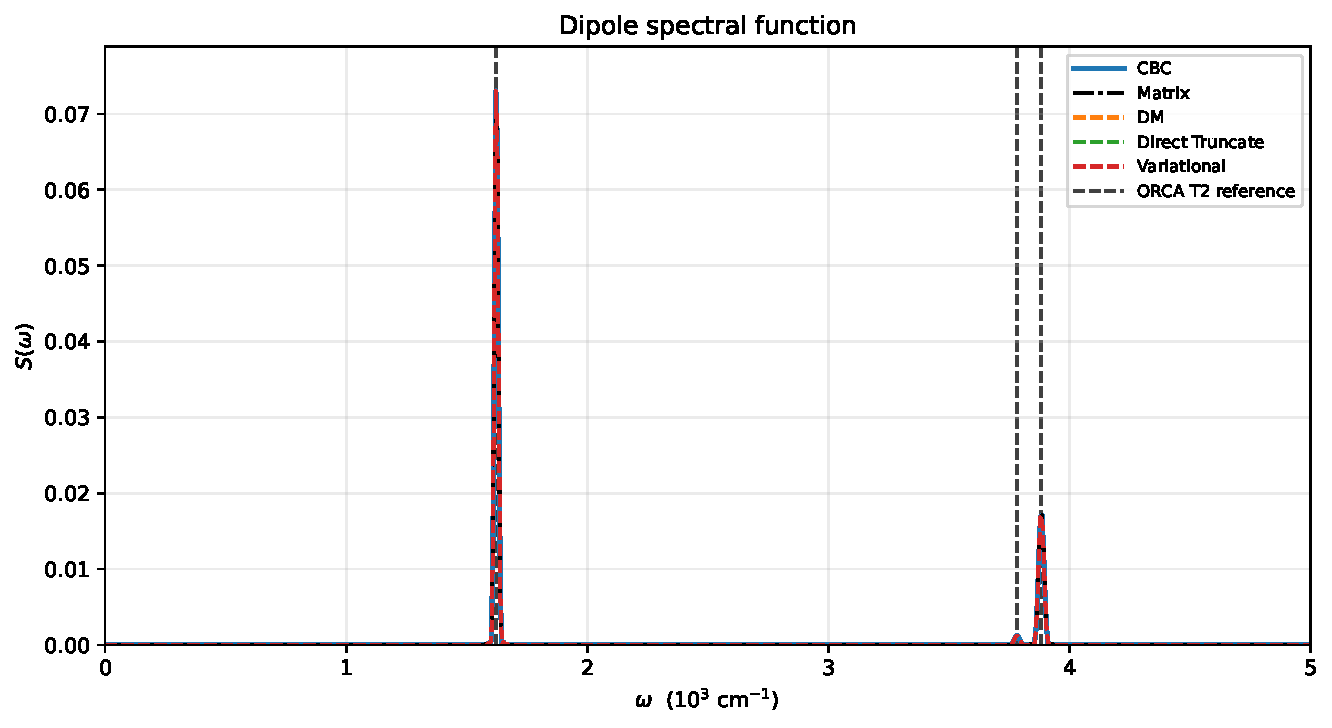
\includegraphics[width=0.95\textwidth]
    {h2o_harmonic_dipole_spectral_function.pdf}
    \caption{
    Dipole spectral function of harmonic H$_2$O calculated with
    \(\chi_{\max}=12\), \(N=125\), and \(N_r=6000\). Results obtained using
    CBC, DM, direct truncation, variational compression, and the dense matrix
    calculation are compared with the ORCA harmonic transition positions.
    }
    \label{fig:h2o_harmonic_chebyshev_spectral_function}
\end{figure}

To compare the spectral weights quantitatively, the integrated IR
intensities obtained from the Chebyshev spectra were compared with the ORCA
harmonic IR intensities. The ORCA reference intensities for the three
transitions are \(77.477\), \(4.093\), and
\(60.559~\mathrm{km\,mol^{-1}}\). For method \(m\), the absolute
percentage error for transition \(f\) is defined as
\begin{equation}
    \epsilon_f^{(m)}
    =
    \frac{
        \left|
        A_{f,N}^{\mathrm{IR}}
        -
        A_f^{\mathrm{IR,ORCA}}
        \right|
    }{
        A_f^{\mathrm{IR,ORCA}}
    }
    \times 100\% ,
    \label{eq:h2o_ir_intensity_error}
\end{equation}
where \(A_{f,N}^{\mathrm{IR}}\) is the intensity obtained from the
Chebyshev spectrum and \(A_f^{\mathrm{IR,ORCA}}\) is the corresponding ORCA
harmonic reference value. The mean error is
\begin{equation}
    \overline{\epsilon}^{(m)}
    =
    \frac{1}{3}
    \sum_{f=1}^{3}
    \epsilon_f^{(m)} .
    \label{eq:h2o_mean_ir_intensity_error}
\end{equation}

The intensity errors are shown in
Figure~\ref{fig:h2o_harmonic_ir_intensity_error}. For all five calculations,
the errors for the three transitions are \(0.444\%\), \(0.370\%\), and
\(0.414\%\), respectively. The corresponding mean error is
\(0.409\%\) for CBC, DM, direct truncation, variational compression, and the
dense matrix calculation. The equality of the errors confirms that, for this
harmonic H$_2$O benchmark, the remaining deviation from the ORCA intensities
is dominated by the finite Chebyshev reconstruction and the numerical
integration of the broadened peaks rather than by the tensor-network
compression method.

\begin{figure}[t]
    \centering
    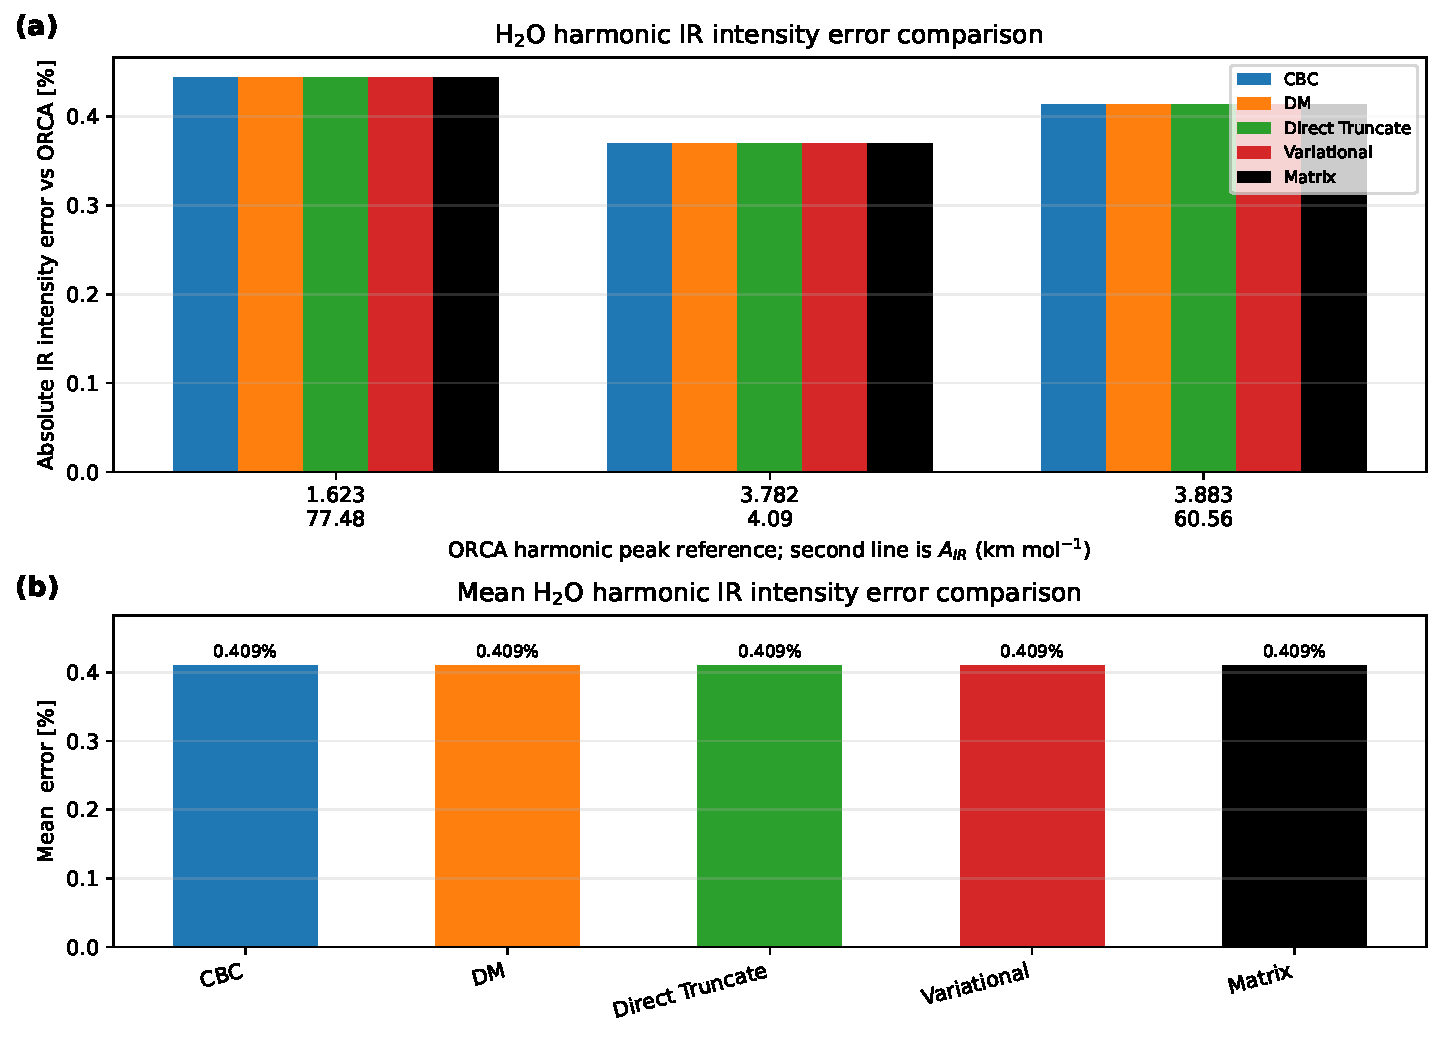
\includegraphics[width=\textwidth]
    {h2o_harmonic_ir_intensity_error_panels_ab.pdf}
    \caption{
    Comparison of the harmonic H$_2$O IR intensity errors.
    (a) Absolute percentage errors relative to the ORCA harmonic intensities
    for the three vibrational transitions. The first line below each group
    gives the transition position in units of \(10^{3}~\mathrm{cm}^{-1}\),
    while the second line gives the corresponding ORCA intensity in
    \(\mathrm{km\,mol^{-1}}\).
    (b) Mean IR intensity error for each method.
    }
    \label{fig:h2o_harmonic_ir_intensity_error}
\end{figure}

Overall, the harmonic H$_2$O calculation shows that all four
tensor-network compression methods reproduce the dense matrix Chebyshev
spectrum and the ORCA harmonic intensities with essentially the same
accuracy. The mean IR intensity error is about \(0.4\%\) for all methods,
indicating that the Chebyshev reconstruction is well converged for this
small harmonic benchmark.
